\section*{Exercise 4}
\subsection*{a)}\small The Certer is underlined.\normalsize

\paragraph{Round 1}~\newline
Cluster 1: $\underline{A}$\\
Cluster 2: $\underline{B}$\\
Cluster 3: $\underline{C},D,E,F,G,H$

\paragraph{Round 2}~\newline
Cluster 1: $\underline{A}$\\
Cluster 2: $\underline{B},C$\\
Cluster 3: $\underline{(7.5,6)},D,E,F,G,H$

\paragraph{Round 3}~\newline
Cluster 1: $\underline{A},B$\\
Cluster 2: $\underline{(3,9.5)},C$\\
Cluster 3: $\underline{(8.5,5.6)},D,E,F,G,H$

\paragraph{Round 4}~\newline
Cluster 1: $\underline{(3.5,11.5)},A,B$\\
Cluster 2: $\underline{C}$\\
Cluster 3: $\underline{(8.5,5.6)},D,E,F,G,H$\\
The clustering of the Points stays the same as the roud before so the algorithm halts.

\subsection*{b)}
\begin{center}
  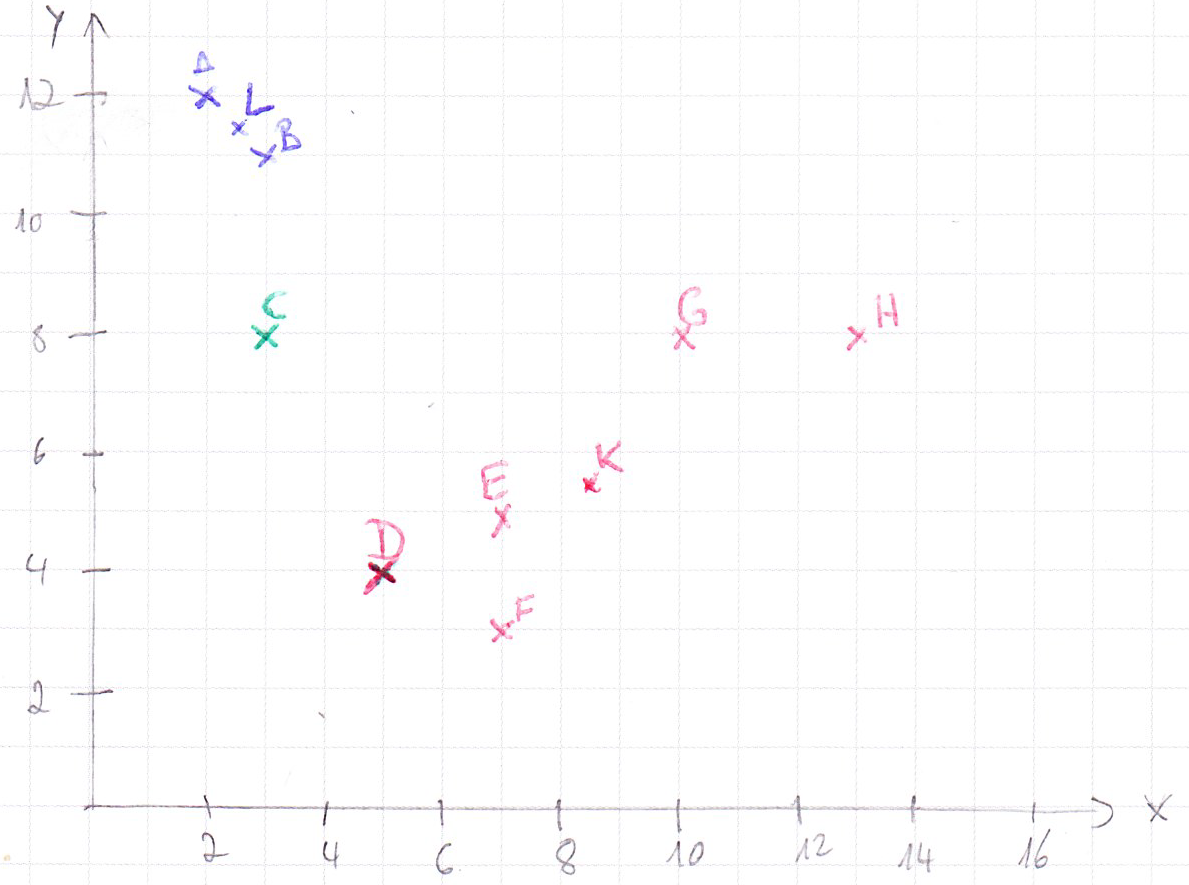
\includegraphics[width=0.7\linewidth]{E4_diag}\\
  \small $L$ is mean of cluster 1: $(2.5,11.5)$, $C$ is mean of cluster 2: $(3,8)$, K is mean of cluster 3: $(8.5,5.6)$
\end{center}

The dividing lines between the clusters are the lines that contain all points with the same distance to two of the points.

So the line seperating the clusters with mean A and B are defined by 
  \[||\left(x,f(x)\right)-A|| = ||\left(x,f(x)\right)-B||\]\\
  \[\Leftrightarrow ||(x-A_1,f(x)-A_2)||=||(x-B_1,f(x)-B_2)||\]\\
  \[\Leftrightarrow \sqrt{(x-A_1)^2 + (f(x)-A_2)^2}=\sqrt{(x-B_1)^2 + (f(x)-B_2)^2}\]\\
  \[\Leftrightarrow (x-A_1)^2 + (f(x)-A_2)^2=(x-B_1)^2 + (f(x)-B_2)^2\]\\
  \[\Leftrightarrow f(x) = \frac{(x-A_1)^2-(x-B_1)^2-A_2^2-B_2^2}{2(A_2-B_2)}\]\\
  \[\Leftrightarrow f(x) = \frac{B_1-A_1}{A_2-B_2}x +\frac{A_1^2+B_1^2-A_2^2-B_2^2}{2(A_2-B_2)}\]\\
  
  The seperation of the clusters can be described by three functions:\\
  Cluster 1\&2: $f(x) = 1/7x+\frac{181}{7}$\\
  Cluster 2\&3: $f(x) = \frac{11}{4.8}x+\frac{14.11}{4.8}$\\
  Cluster 1\&3: $f(x) = \frac{12}{11.8}x+\frac{85.11}{11.8}$
  
\subsection*{c)}
Choosa $A,F$ and $H$ as initial cluster means.
\[||B-A||=\sqrt{2}, ||C-A||=\sqrt{17} \rightarrow A, ||D-A||=\sqrt{73}, ||E-A||=\sqrt{74},||G-A||=4\sqrt{5}\]\\
\[||B-F||=4\sqrt{5}, ||C-F||=\sqrt{41}, ||D-F||=\sqrt{5} \rightarrow F, ||E-F||=2\rightarrow F,||G-F||=\sqrt{34}\]\\
\[||B-H||=\sqrt{109}, ||C-H||=10 \rightarrow A, ||D-H||=4\sqrt{5}, ||E-H||=3\sqrt{5},||G-H||=3\rightarrow H\]\\
Cluster 1: $\underline{A},B,C$ \hfill \small Center is underlined\\
Cluster 2: $D,E,\underline{F}$\\
Cluster 3: $G,\underline{H}$\\
Using $z^j\leftarrow\frac{\sum_{x\in C^j}x}{|C^j|}$ the new centroids are:
$C_1: (2.667,10.333), C_2: (6.333,4), C_3: (11.5,8)$.\\
Using the new centroids leads to the following clusters:\\
$C_1:\underline{(2.667,10.333)},A,B,C$\\
$C_2:\underline{(6.333,4)},D,E,F$\\
$C_3:\underline{(11.5,8)},G,H$\\
Th clusters are the same as in the prevois step so thete starting centroids produce a different result than a).
\subsection*{d)}
\[||A-G||=4\sqrt{5}, ||B-G|| = \sqrt{58}, ||B-A||=\sqrt{2}\]
The shortest distance of all the points to eachother is the distance between A and B. So A and B have to be in a cluster except A and B are centers of a cluster each. Then the distance between A and G is longer then B ang G.
Therfore G would be in the cluster of B.
It's impossible for k-means to return $\lbrace A,G\rbrace$ as a cluster.